% Suggested insertion for Section 3.2, after the alpha-sensitivity or finite-precision paragraph.

\paragraph*{Order-dependent finite-precision effect near $\alpha=2$.}
The preceding $\alpha$-sweep also reveals a subtle point: even for Gauss--Jacobi quadrature, the raw quotient error may increase as $\alpha\to2$.  To determine whether this behavior is due to the quadrature rule or to floating-point evaluation of the endpoint quotients, we repeat the Gauss--Jacobi $\alpha$-sweep for the smooth benchmark $f(t)=e^{-t}$, $t=1.5$, and $M=100$, while evaluating the raw quotients under fp64, fp32, fp16 and fp8-like quantization.  The fp8-like curves use e5m2/e4m3 quantization diagnostics and are not intended to model a complete mixed-precision training pipeline.

\begin{figure}[htbp]
    \centering
    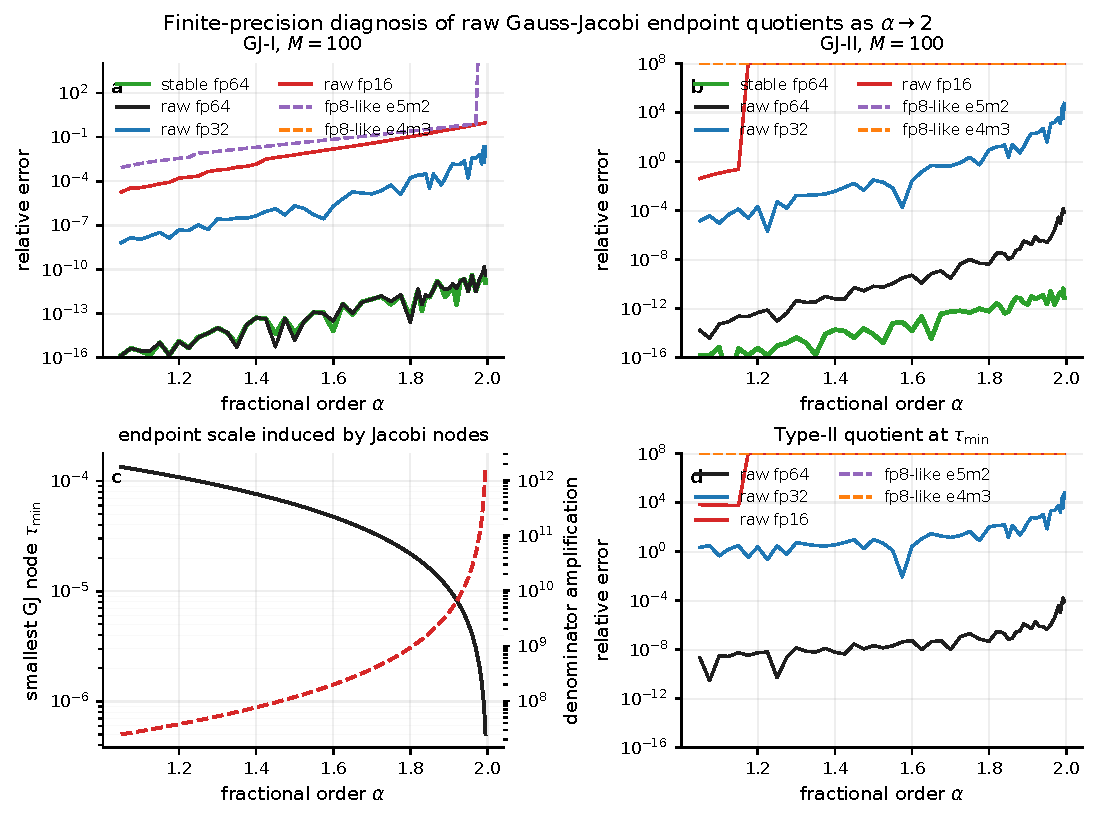
\includegraphics[width=0.95\textwidth]{figures/fig12_alpha2_gj_precision_sweep.pdf}
    \caption{Finite-precision diagnosis of raw Gauss--Jacobi endpoint quotients as $\alpha\to2$ for $f(t)=e^{-t}$, $t=1.5$, and $M=100$.  Stable fp64 uses algebraically equivalent \texttt{expm1}/Taylor endpoint formulas.  The raw fp64 Type-II error increases near $\alpha=2$, fp32 deteriorates much earlier, and fp16/fp8-like evaluations enter overflow or invalid regimes.  The lower-left panel shows that the leftmost node approaches $\tau=0$ as $\alpha\to2$, increasing the denominator amplification $(t\tau_{\min})^{-2}$.}
    \label{fig:valid-alpha2-precision}
\end{figure}

\begin{table}[htbp]
\centering
\caption{Relative GJ-II errors as $\alpha\to2$ under different quotient-evaluation precisions.  The final two columns report the relative error of the local Type-II quotient at the smallest Gauss--Jacobi node.  Values marked overflow/NaN indicate that the quantized denominator or numerator evaluation became invalid.}
\label{tab:valid-alpha2-precision}
\begin{tabular}{c|cc|ccccc|cc}
\hline
$\alpha$ & $\tau_{\min}$ & $(t\tau_{\min})^{-2}$ & stable fp64 & raw fp64 & raw fp32 & raw fp16 & fp8-like e5m2 & local q2 fp64 & local q2 fp32 \\
\hline
$1.25$ & $9.99\times10^{-5}$ & $4.46\times10^{7}$  & $9.61\times10^{-16}$ & $9.85\times10^{-14}$ & $5.30\times10^{-4}$ & overflow/NaN & overflow/NaN & $5.28\times10^{-11}$ & $2.93$ \\
$1.50$ & $6.14\times10^{-5}$ & $1.18\times10^{8}$  & $2.35\times10^{-15}$ & $6.89\times10^{-11}$ & $3.21\times10^{-2}$ & overflow/NaN & overflow/NaN & $2.19\times10^{-8}$  & $9.98$ \\
$1.75$ & $2.79\times10^{-5}$ & $5.69\times10^{8}$  & $1.12\times10^{-13}$ & $1.05\times10^{-8}$  & $2.33$              & overflow/NaN & overflow/NaN & $2.03\times10^{-7}$  & $4.49\times10^{1}$ \\
$1.90$ & $1.05\times10^{-5}$ & $4.05\times10^{9}$  & $2.16\times10^{-12}$ & $2.56\times10^{-7}$  & $6.81\times10^{1}$ & overflow/NaN & overflow/NaN & $8.70\times10^{-7}$  & $2.32\times10^{2}$ \\
$1.98$ & $2.02\times10^{-6}$ & $1.09\times10^{11}$ & $1.20\times10^{-11}$ & $2.93\times10^{-5}$  & $4.08\times10^{3}$ & overflow/NaN & overflow/NaN & $3.77\times10^{-5}$  & $5.25\times10^{3}$ \\
$1.99$ & $1.00\times10^{-6}$ & $4.40\times10^{11}$ & $1.19\times10^{-11}$ & $8.75\times10^{-5}$  & $2.96\times10^{4}$ & overflow/NaN & overflow/NaN & $9.93\times10^{-5}$  & $3.36\times10^{4}$ \\
\hline
\end{tabular}
\end{table}

\begin{remark}[Raw Gauss--Jacobi quotients near $\alpha=2$]
The increase of raw Gauss--Jacobi errors near $\alpha=2$ is an implementation-level finite-precision effect rather than a failure of the quadrature rule.  In the Type-II formula, the quotient
\[
    \frac{f(t)-f(t-h)-h f'(t)}{h^2},\qquad h=t\tau,
\]
forms an $O(h^2)$ numerator by subtracting $O(1)$ quantities and then divides by $h^2$.  As $\alpha\to2$, the Jacobi exponent $1-\alpha\to-1$, and the left endpoint nodes move closer to $\tau=0$.  Therefore, raw endpoint quotients become increasingly roundoff-sensitive.  For smooth benchmarks, this sensitivity is removed by algebraically stable endpoint evaluation, for example by using \texttt{expm1} and Taylor replacement near $h=0$.  Hence large errors from raw low-precision quotients should be interpreted as endpoint-cancellation artifacts, not as contradictions of the Gauss--Jacobi convergence theorem for exactly evaluated smooth kernels.
\end{remark}
